\hypertarget{brushfire-algorithm}{%
\section{Brushfire Algorithm}\label{brushfire-algorithm}}

The \texttt{Brushfire\ algorithm} is used to compute the distances which
are used in the repulsive potential. \emph{It is not a planner!.} It
will replace the \(d(p,q)\) function above and can be part of other
planning algorithms. Assume that your map is represented on a grid
domain.

\begin{figure}
\centering
\includegraphics[width=0.35\textwidth,height=\textheight]{PlanningFigures/griddomain.png}
\caption{A grid domain with obstacles. Normal practice is to label the
cell as occupied if any part of the physical obstacle overlaps the
cell.}
\end{figure}

\begin{figure}
\centering
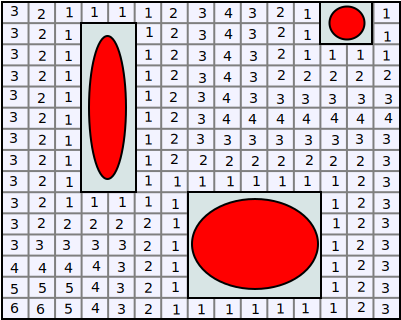
\includegraphics[width=0.35\textwidth,height=\textheight]{PlanningFigures/brushfire.*}
\caption{Example of obstacle overlab with grid domain.}
\end{figure}

\begin{figure}
\centering
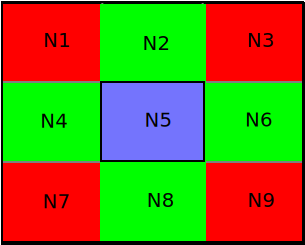
\includegraphics[width=0.35\textwidth,height=\textheight]{PlanningFigures/neighbors2.*}
\caption{Four and eight point connectivity to determine neighbors.}
\end{figure}

Four point neighbors have a distance which is the same as the Euclidean
distance. Eight point connectivity includes diagonals, greater
connectivity, but ignores diagonal distance.

\begin{itemize}
\tightlist
\item
  Set free space pixels to zero.
\item
  Set pixels which are occupied, even partially, by objects to 1
\item
  Neighbor pixels (containing 0) to object pixels are set to 2
\item
  Neighbors (containing 0) to pixels containing 2 set to 3, etc
\end{itemize}

Gradient map made by looking at the smallest value in your connectivity.

\begin{quote}
Brushfire example
\end{quote}

A gradient map can be produced at each pixel by finding the neighbor
pixel with the largest value. Both distance and gradient are now
available and thus a planning algorithm can use this to determine a
path. \texttt{fig:SteepestDescentPath} shows the Steepest Descent Path.
This path may not be unique due to the discrete nature of the domain
map. At each step, there can be multiple cells with the same value. One
must have a selection process and different selection choices lead to
different descent paths. Note that this process will generalize to any
dimension.

\begin{quote}
Steepest Descent Path
\end{quote}

\hypertarget{potentials-and-brushfire}{%
\subsection{Potentials and Brushfire}\label{potentials-and-brushfire}}

The Brushfire algorithm may be used to replace the repulsive potential.
The attractive potential is still required to complete the routing. One
may use any form of attractive potential. The idea is to use the
atttractive potential to direct the robot to the goal. The Brushfire
algorithm can be used to keep the robot from colliding with an obstacle.
Since the Brushfire map includes distance to an obstacle, then the cells
of greatest increase are in the direction away from the obstacle. This
is a discrete negative gradient. In combination with the attractive
potential can be used to route.

\begin{figure}
\centering
\includegraphics[width=0.5\textwidth,height=\textheight]{PlanningFigures/brushfiresurface.png}
\caption{Brushfire Surface}
\end{figure}

One approach to planning is given in Algorithm
\href{..\%20topic::\%20\%20Discrete\%20potential\%20function\%20planner}{alg:brushfire}.
Assume that the domain is discretized and the current location of the
robot is indexed by \(q = (i,j)\). Also assume the goal location is
\(q_{\text{goal}} = (i^*,j^*)\). Call the Brushfire cell number for cell
\(q = (i,j)\), \(b(q)\). The attractive potential in grid coordinates is
\(U = [(i-i^*)^2 + (j-j^*)^2]/2\), so the gradient
\(\nabla U =  (i-i^*,j-j^*) = q - q_{\text{goal}}\). We can combine
Brushfire with the discrete potential function to obtain the Algorithm
\href{..\%20topic::\%20\%20Discrete\%20potential\%20function\%20planner}{alg:brushfire}.

\begin{quote}
\textbf{Input} A point robot with a tactile sensor and
\(D_\text{min}\).\\
\textbf{Output} A path to the goal.\\
\textbf{while} true \textbf{do}\\
\hspace*{0.333em}\hspace*{0.333em}*\emph{repeat}*\\
\hspace*{0.333em}\hspace*{0.333em}\hspace*{0.333em}\hspace*{0.333em}Compute
\(q_{\text{goal}}-q = (h,k)\).\\
\hspace*{0.333em}\hspace*{0.333em}\hspace*{0.333em}\hspace*{0.333em}Compute
\(z = \text{max}(h,k)\) and
\(\Delta q =  (\text{int } h/z, \text{int } k/z)\)\\
\hspace*{0.333em}\hspace*{0.333em}\hspace*{0.333em}\hspace*{0.333em}Compute
\(q_{\text{new}} = q + \Delta q\)\\
\hspace*{0.333em}\hspace*{0.333em}\hspace*{0.333em}\hspace*{0.333em}Set
\(q_{\text{new}} \to q\)\\
\hspace*{0.333em}\hspace*{0.333em}*\emph{until}* \(q = q_{\text{goal}}\)
or \(b(q) = D_\text{min}\)\\
\textbf{if} Goal is reached\\
\textbf{then} exit\\
Set \(L\) equal to list of unvisited neighbor cells with
\(b(i,j) = D_\text{min}\)\\
\textbf{if} L is empty, \textbf{then} conclude there is no path to
goal.\\
\textbf{repeat}\\
\hspace*{0.333em}\hspace*{0.333em}Select \(q = (i,j) \in L\)\\
\hspace*{0.333em}\hspace*{0.333em}Compute
\(q_{\text{goal}}-q = (h,k)\).\\
\hspace*{0.333em}\hspace*{0.333em}Compute \(z = \text{max}(h,k)\) and
\(\Delta q =  (\text{int } h/z, \text{int } k/z)\)\\
\hspace*{0.333em}\hspace*{0.333em}Compute
\(q_{\text{new}} = q + \Delta q\)\\
\hspace*{0.333em}\hspace*{0.333em}Set \(L\) equal to list of unvisited
neighbor cells with \(b(i,j) = D_\text{min}\)\\
\hspace*{0.333em}\hspace*{0.333em}*\emph{if}* L is empty, \textbf{then}
conclude there is no path to goal.\\
\textbf{until} \(q_{\text{goal}}\) is reached or
\(b(q_{\text{new}}) > D_\text{min}\)
\end{quote}

\hypertarget{dealing-with-discrete-functions}{%
\subsection{Dealing with discrete
functions}\label{dealing-with-discrete-functions}}

How do we modify the potential function approach? Recall that we have

\[U(q) = U_\text{att}(q) + U_\text{rep}(q)\]

with the attractive potential as

\[\begin{aligned}
U_\text{att}(q) = \left\{ \begin{array}{ll} (1/2)\gamma d^2(q, q_\text{goal}), & d(q, q_\text{goal})\leq d^*_\text{goal},\\[3mm]
d^*_\text{goal}\gamma d(q, q_\text{goal}) - (1/2)\gamma (d^*_\text{goal})^2, & d(q, q_\text{goal})> d^*_\text{goal},
\end{array}\right.
\end{aligned}\]

and the repulsive potential as

\[\begin{aligned}
U_\text{rep}(q) = \left\{ \begin{array}{ll} (1/2)\eta \left( \frac{1}{\tilde{D}(q)} - \frac{1}{Q^*}\right) , &
\tilde{D}(q) \leq Q^*,\\[3mm]
0, & \tilde{D}(q) > Q^*
\end{array}\right.
\end{aligned}\]

where \(\tilde{D}\) is found from the Brushfire Map. The issue is that
\(\tilde{D}\) is not a continuous function. It is a piecewise constant
function and so \(\nabla \tilde{D}\) is zero on all of the interiors of
the cells.\footnote{Known as zero "almost everywhere".}

\begin{figure}
\centering
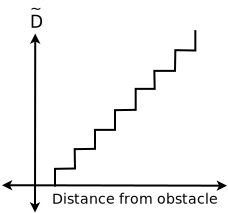
\includegraphics[width=0.4\textwidth,height=\textheight]{PlanningFigures/piecewise_const.*}
\caption{}
\end{figure}

The gradient can be estimated as the difference in cell values. Thus

\[\nabla U_{rep}  = \left< \Delta \tilde{D} / \Delta x , \Delta  \tilde{D} / \Delta y \right>\]

Because the discrete distance function jumps, it can cause the path to
oscillate back and forth along the normal direction to the
obstacle.\footnote{This is due to the switching on and off a large
  repulsive potential.} Tuning the potential function can also be
challenging. One may need to adjust weights in the sum:

\[aU_\text{att}(q) + bU_\text{rep}(q)\]

What one wants is motion orthogonal to the boundary of the obstacle.

Motion towards the obstacle is in the direction of the repulsive
potential gradient, \(\nabla U_\text{rep}\), so we select motion
orthogonal to the gradient, \(\nabla U_\text{rep}^{\perp}\):

\[\mbox{Heading} = \lambda (1-d) \nabla U_\text{att} + \lambda d \nabla U_\text{rep}^{\perp}\]

where \(d = D/Q^*\) and \(\lambda\) is positive ``tunable" value. This
gives a smooth transition to orthogonal motion. We still need to
understand \(\nabla U_\text{rep}^{\perp}\).

The orthogonal subspace \(\nabla U_\text{rep}^{\perp}\) is a line. From
this we need to select a direction. We can do this by projecting the
gradient of the attractive potential onto the subspace:

\[\mbox{proj}(\nabla U_\text{att})_{\nabla U_\text{rep}^{\perp}} =
\displaystyle \frac{\left(\frac{\partial U_\text{att}}{\partial x}\right)\left(\frac{\partial U_\text{rep}}{\partial y}\right)- \left(\frac{\partial U_\text{att}}{\partial y}\right)\left(\frac{\partial U_\text{rep}}{\partial x}\right) }
{ \| \nabla U_\text{rep}\|^2} \nabla U_\text{att} .\]

\hypertarget{local-minima-problem}{%
\subsection{Local Minima Problem}\label{local-minima-problem}}

Gradient descent will move towards a local minimum, but not necessarily
the global minimum. Take the map with goal given by
\texttt{potentialwell}.

\begin{quote}
Using an attractive potential function centered at the goal and a
repulsive potential function based on distance from the obstacle, the
robot will be attracted to some point \emph{x} where it will stop. This
point is a local minimum in the combined potential function (attractive
and repulsive potentials combined).
\end{quote}

There is a point, \emph{x} inside the horseshoe where the attractive
forces and repulsive forces balance giving rise to a local min for the
combined potential function. The robot will stall at this point. There
is not a simple fix here.

\hypertarget{maximum-obstacle-distance-path}{%
\subsection{Maximum obstacle distance
path}\label{maximum-obstacle-distance-path}}

Some routing problems require the vehicle to keep a maximum distance
from obstacles. For example, quadrotors are effected by ground and wall
effects which can cause collisions and vehicle damage. Using the
Brushfire and Wavefront algorithms together can be used to produce safe
paths. The idea is to use the Brushfire algorithm to do the
skeletalization of the domain. Then the Wavefromt algorithm searches the
reduced path.

\begin{itemize}
\tightlist
\item
  Use Brushfire to find equidistance points or ridges and label ridge
  pixels
\item
  Compute shortest path between start point and the ridge: start path

  \begin{itemize}
  \tightlist
  \item
    Use a Wavefront planner.
  \item
    Set the start point as the wave start.
  \item
    Stop when the wave hits the ridge.
  \item
    Label start path pixels
  \end{itemize}
\item
  Compute shortest path between end point and the ridge: end path

  \begin{itemize}
  \tightlist
  \item
    Use a Wavefront planner.
  \item
    Set the end point as the wave start.
  \item
    Stop when the wave hits the ridge.
  \item
    Label end path pixels.
  \end{itemize}
\item
  Back track along different segments in the path list to find global
  path

  \begin{itemize}
  \tightlist
  \item
    Starting at end pixel.
  \item
    Apply wavefront to labeled pixels.
  \item
    Stop wavefront when start pixel is found.
  \end{itemize}
\end{itemize}

\textbf{Footnotes}
